\documentclass[conference]{IEEEtran}
\IEEEoverridecommandlockouts

\usepackage{cite}
\usepackage{amsmath,amssymb,amsfonts}
\usepackage{algorithmic}
\usepackage{graphicx}
\usepackage{textcomp}
\usepackage{xcolor}
\usepackage{listings}
\graphicspath{ {./images/} }
\def\BibTeX{{\rm B\kern-.05em{\sc i\kern-.025em b}\kern-.08em
    T\kern-.1667em\lower.7ex\hbox{E}\kern-.125emX}}
\begin{document}

\title{Pathline of 32-RISC ISA\\}

\author{\IEEEauthorblockN{Martin Carrasco}
\IEEEauthorblockA{\textit{Computer Science} \\
\textit{UTEC}\\
Lima, Peru \\
martin.carrasco@utec.edu.pe}
\and
\IEEEauthorblockN{Andrea Diaz}
\IEEEauthorblockA{\textit{Computer Science} \\
\textit{UTEC}\\
Lima, Peru \\
andrea.diaz@utec.edu.pe}
}
\maketitle

\begin{abstract}
This document describes the procedure of creating a 32 bits MIPS processor in Verilog, the program is designed to execute basic algorithms with a pre-defined short set of instructions. We will describe the methods we used to create it, the input and outputs of every module and a brief description of the individual function of each of them.
\end{abstract}

\begin{IEEEkeywords}
MIPS processor, Verilog, ISA, Datapath, RISC
\end{IEEEkeywords}

\section{Introduction}
Everything in the processor starts with the decomposition of high-level languages to something more understandable to a computer, this happens with the help of the instruction set architecture (ISA). The ISA act as a main schematic for how the machine will work. To improve the process of translation to machine language was first introduced the reduced instruction set computer (RISC) technology. Enlisting the most used operations and minimizing them in a way that simple instructions can be combined to form complex statements. This architecture can run three times faster than others because of this. language. The assembler-compiler ratio is the
execution time for an assembler program divided by the exe?
cution time for a compiled version of the program. This ratio is
less than 50 percent for CISCs. For the RISC II, however, it is 90
percent.\cite{10.2307/29774812} Nowadays, most universities and research labs use MIPS, one of the first RISC architectures, as their favorite;  the simplicity of it makes it easier to manage the size of the RISC code. With simplicity

\subsection{MIPS - instructions}
Every computer executes a pre-established set of instructions. These instructions are organized into five different types. The three main ones that we will use in this paper are  R-type[Table \ref{tab1}] performs simple arithmetic and logic operations, the I-type[Table \ref{tab2}], immediate values and a register values; and the J-type[Table \ref{tab3}], jumps.
MIPS has a vast number of instructions, but for the purpose of simplification, we will only use the following in the Table \ref{tab4}.

    \begin{table}[htbp]
    \caption{R-type format}
    \begin{center}
    \begin{tabular}{|c|c|c|c|c|c|}
    \hline
    \multicolumn{6}{|c|}{R-type fields}                 \\ \hline
    op     & rs     & rt     & rd     & shamt  & funct  \\ \hline
    6 bits & 5 bits & 5 bits & 5 bits & 5 bits & 6 bits \\ \hline
    \end{tabular}
    \label{tab1}
    \end{center}
    \end{table}
    
    \begin{table}[htbp]
    \caption{I-type format}
    \begin{center}
    \begin{tabular}{|c|c|c|c|}
    \hline
    \multicolumn{4}{|c|}{I-type fields}  \\ \hline
    op     & rs     & rt     & inmediate \\ \hline
    6 bits & 5 bits & 5 bits & 16 bits   \\ \hline
    \end{tabular}
    \label{tab2}
    \end{center}
    \end{table}
    
    \begin{table}[htbp]
    \caption{J-type format}
    \begin{center}
    \begin{tabular}{|c|c|}
    \hline
    \multicolumn{2}{|c|}{J-type} \\ \hline
    op & offset \\ \hline
    \end{tabular}
    \label{tab3}
    \end{center}
    \end{table}
    
    \begin{table}[htbp]
    \caption{Instructions supported by our MIPS}
    \begin{center}
    \begin{tabular}{cc|c|c}
    \hline
    \multicolumn{1}{|c|}{R-type} & \multicolumn{2}{c|}{I-type} & \multicolumn{1}{c|}{J-type} \\ \hline
    \multicolumn{1}{|c|}{add} & addi & \multicolumn{1}{c|}{lb} & \multicolumn{1}{c|}{j} \\ \hline
    \multicolumn{1}{|c|}{sub} & subi & \multicolumn{1}{c|}{lh} & \multicolumn{1}{c|}{jr} \\ \hline
    \multicolumn{1}{|c|}{and} & andi & \multicolumn{1}{c|}{lw} & \multicolumn{1}{c|}{jal} \\ \hline
    \multicolumn{1}{|c|}{nor} & ori & \multicolumn{1}{c|}{sb} &  \\ \cline{1-3}
    \multicolumn{1}{|c|}{or} & slti & \multicolumn{1}{c|}{sh} &  \\ \cline{1-3}
    \multicolumn{1}{|c|}{slt} & beq & \multicolumn{1}{c|}{sw} &  \\ \cline{1-3}
    \multicolumn{1}{|c|}{} & bneq & \multicolumn{1}{c|}{lui} &  \\ \cline{1-3}
    \multicolumn{1}{l|}{} & \multicolumn{1}{l|}{bgez} & \multicolumn{1}{l}{} & \multicolumn{1}{l}{} \\ \cline{2-2}
    \end{tabular}
    \label{tab4}
    \end{center}
    \end{table}
    
\subsection{Datapath}
The MIPS implementation[Fig. \ref{fig:datapath}] goes into a graphic model called datapath, every component works in a different way, between decoding the instruction and passing it to the next one, the processor can have a big amount of tasks that influence on the final performance.

    \begin{figure}[h]
    \caption{Control and datapath that handles the jump instruction}
    \centering
    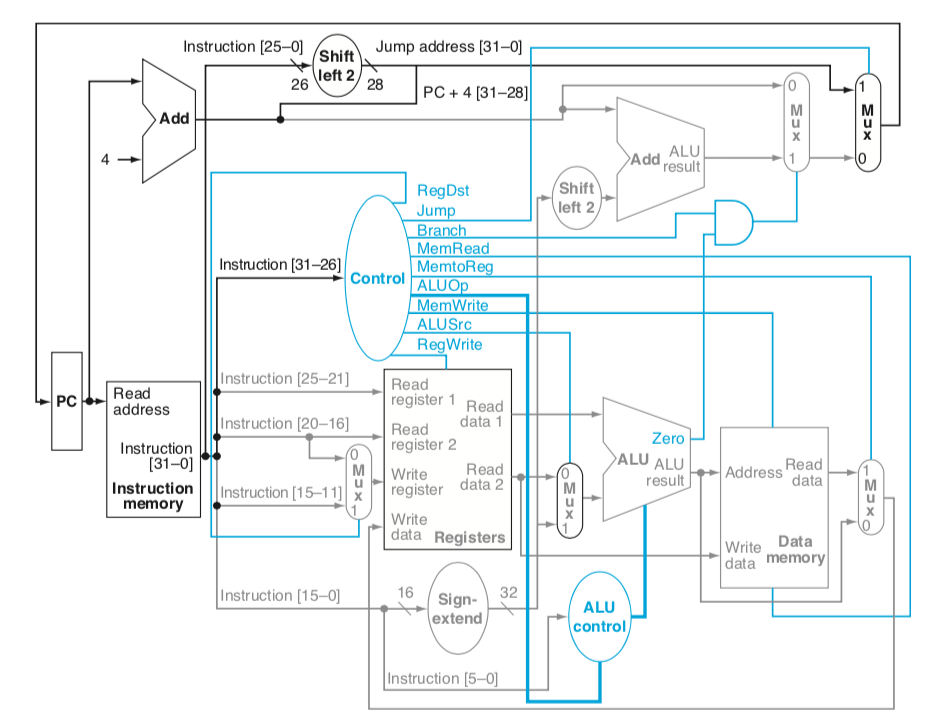
\includegraphics[scale=0.5]{images/datapath.png}
    \label{fig:datapath}
    \end{figure}
    

\section{Methodology}
For the construction and designing of the processor we used Verilog as our hardware description language, Icarus Verilog as simulation and synthesis tool, and Scansion as our main simulator with the alternated use of GTKWave and ModelSim.
    
    \subsection{The coding}
    We started with the simple modules (mux, shift left, sign extend, the adders and the AND used for the branch)  then we continued to the more complex sections. All the modules were first made without linking and the variables wrote to resemble the input and outputs of the datapath show on the Figure \ref{fig:datapath}, but after more implementations some of them alternated.
    
    \subsection{Principal Modules}
    The biggest code was the control, but the hardest procedure was the code for the implementation of the datapath file that we named Datapath.v; this is in charge of delivering the wires for each module, setting up the clock of the processor and linking every variable that needs to be send between units.
    

    \begin{figure}[h]
        \caption{Fetching instruction. The Program counter, Instruction Memory and a Add 4}
        \centering
        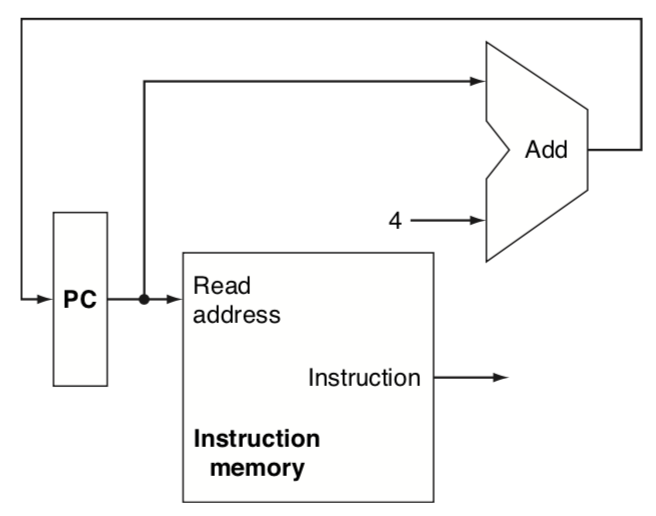
\includegraphics[scale=0.5]{images/fetching-ins.png}
        \label{fig:Fetching-ins}
    \end{figure}
    

\section{Experimental Setup}

\subsection{Program Counter}
    Every instruction is 32 bits, those go to the instruction memory and to the 4 adder via wires[Fig. \ref{fig:Fetching-ins}]. The program counter is in charge of handing the previous and next instruction, including delivering the branch when the jump is necessary.
    The program counter equation when jump is used
    \[PC = Register + Branch Address\]
    
        In our first Verilog program of the PC received a clock, the address and the add 4 result.
        \begin{lstlisting}
        module PC(clk, pc, target_pc);
    	    input clk;
    	    input [31:0] target_pc;
    	    output reg [31:0] pc;
    
    	    initial  begin
    		    pc = 32'b0;
    	    end
    	
    	    always @ (posedge clk) begin
    		    pc = target_pc;
    	    end
        endmodule
        \end{lstlisting}
        
        One of the main struggles we had was the \textit{always} instruction, initially we thought that writing \textit{always @ (posedge clk)} would make the pc change continuously as the clk cycles were running but that's not what happened at the time of the simulation, the pc was only changing at the first clk posedge but modifying the next values to undefined; as the code continue to simulate with this pc value the some of the variables would change to undefined as well.
        
        \begin{figure}[h]
            \caption{PC module error}
            \centering
            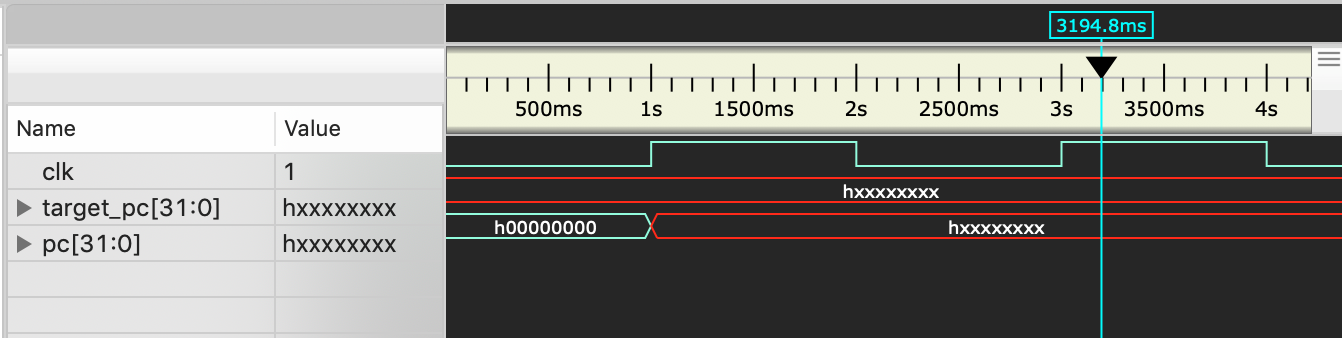
\includegraphics[scale=0.35]{images/pc_error.png}
            \label{fig:pc-error}
        \end{figure}
        
        The temporary solution for this was the \textit{\$display} command of the \textit{target\_pc} (the variable that was allegedly changing the pc) but now the issues was that \textit{\$display} only showed the instant values without waiting for changes to be applied, that quite confused us for a while, after some research and we continued to this command but only to proved the right functionality of the module not anymore to test variable values.\\
        
        PC module fixed
        \begin{lstlisting}
        module PC (clk, pc);
            input clk;
            output reg [31:0] pc;
            
            initial  begin
                pc = 32'b0;
            end
            
            always @ (posedge clk) begin
        	    pc = pc + 32'h4;
            end
        endmodule
        \end{lstlisting}
        We fixed this error by replacing the \textit{target\_pc} by just adding 4 to our pc variable, as a result we removed the  \textit{target\_pc} element as well.

        
        \begin{table}[htbp]
        \caption{Inputs and outputs of the first PC}
        \begin{center}
        \begin{tabular}{|c|c|}
        \hline
        \multicolumn{2}{|c|}{inputs} \\ \hline
        clk & 1 bit \\ \hline
        target\_pc & \multicolumn{1}{l|}{32 bits} \\ \hline
        \multicolumn{2}{|c|}{outputs} \\ \hline
        pc & 32 bits \\ \hline
        \end{tabular}
        \label{tab5}
        \end{center}
        \end{table}
        
        
        
    \subsection{Clock}
    Originally the clock was introduced and defined at our main controller, previously mentioned as DataPath.v, and delivered to every module that need it, the predicament with this way of declaration it was that some units were having their own clocks running in their own pace. The best fix for this inconsistency was to create a new file that is in charge of all the changes in the wave; it had to be changed the inputs and outputs of the modules that used the clk 
    
    
    This is the code for an processor that never stops, for the purpose of only demonstration the clock will run for 50 clicks. 
        \begin{lstlisting}
        module Clock(clk);
            output reg clk;
            
            initial begin
            	clk = 0;
            end
           
            always begin
            	#5 clk <= ~clk;
            end
        endmodule
        \end{lstlisting}
        
        \bigbreak
        Code with 50 click, changing the clock every 5.
        \begin{lstlisting}
        module Clock(clk);
            output reg clk;
            
            initial begin
            	clk = 0;
            end
            
            initial #50 $finish();
            
            always begin
            	#5 clk = ~clk;
            end
        endmodule
        \end{lstlisting}
        
    \begin{figure}[h]
        \caption{Clock module simulation wave}
        \centering
        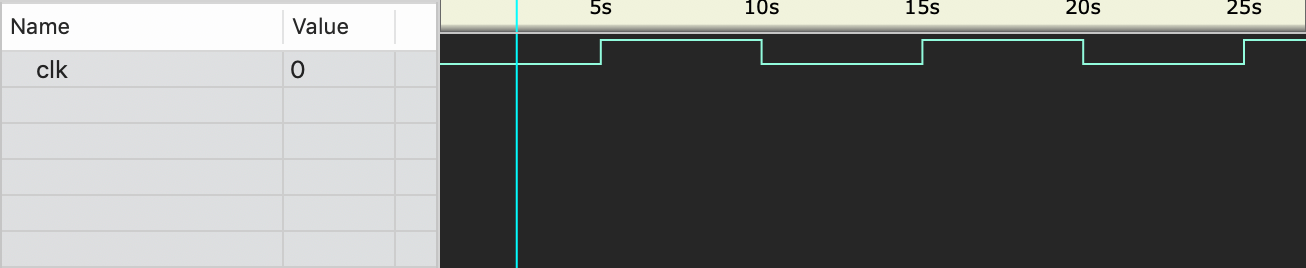
\includegraphics[scale=0.35]{images/clock-module.png}
        \label{fig:clock-wave}
    \end{figure}

    \subsection{Instruction Memory}
    In this module the binary code is divided, the bits from 31 to 26 go to the control and depending of the instruction the rest if bits will be distribute to the register or the sign extend.[Fig. \ref{fig:ins-mem}]
    
    \begin{figure}[h]
        \caption{Our instruction memory reading and addi and an add instruction}
        \centering
        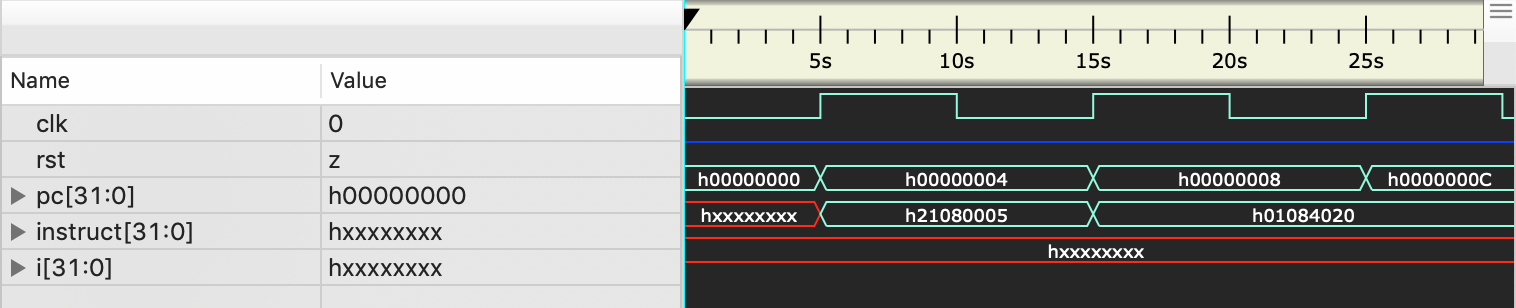
\includegraphics[scale=0.30]{images/instruction-memory.png}
        \label{fig:ins-mem}
    \end{figure}
    
    \subsection{The Data Memory}
    This module represents how we save data to a bigger memory register than the usual register. That is memory we don't use as often as the register but where we need to store larger amounts of data. We can access it in a few different ways. We can either load or save. The sizes we use are word (4bytes), half word(2bytes) or a byte. This works by passing it a a reference to the start of the the array that is memory and and offset for the amount of data.
    
    \subsection{The Registers}
    Here is where all the quasi temporal data is stored and handled. Arguably one of the most important units, here is where every instruction makes a stop to collect or store data. The register is made up of 32 addresses with 1 byte long. Here we store our temporal values, the saved register for the jal instruction, the values we read from memory and everything else we want to operate on to. 
    
    Each set of registers here serves a function some save space for a constant zero (\$0) temporal values (\$t), permanent values (\$s) and some other valuable data we will talk about later on. [Fig. \ref{fig:reg-wave}]
    
    \begin{figure}[h]
        \caption{The register in a simulation of an addi instruction next to a jump one}
        \centering
        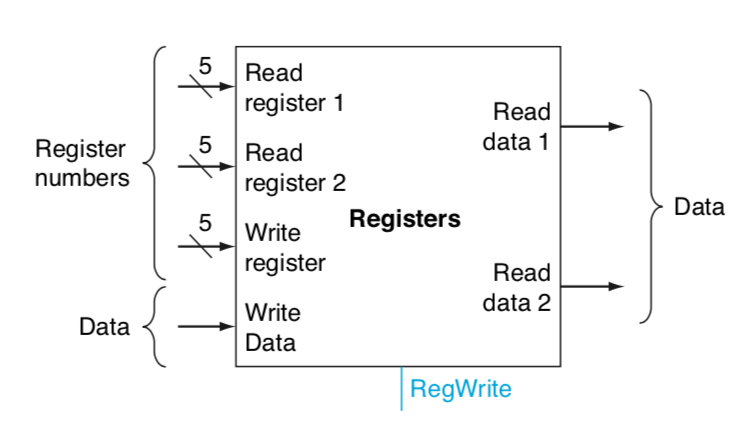
\includegraphics[scale=0.30]{images/registers.png}
        \label{fig:reg-wave}
    \end{figure}
    
    \subsection{The J-type instructions}
    One of our biggest problems was the J-type instructions. When creating the last mux (the one that changed the PC to the address we were jumping) where the output was our \textit{pc wire}, the same one we were passing to the PCModule and, as you can see in the PC module fixed code, by giving the pc wire with a changed value to this module it damaged the rest of the modules that depended of the PC module output [Fig. \ref{fig:jump-mux-error}].
    
    \begin{figure}[h]
        \caption{The simulation with the pc wire error}
        \centering
        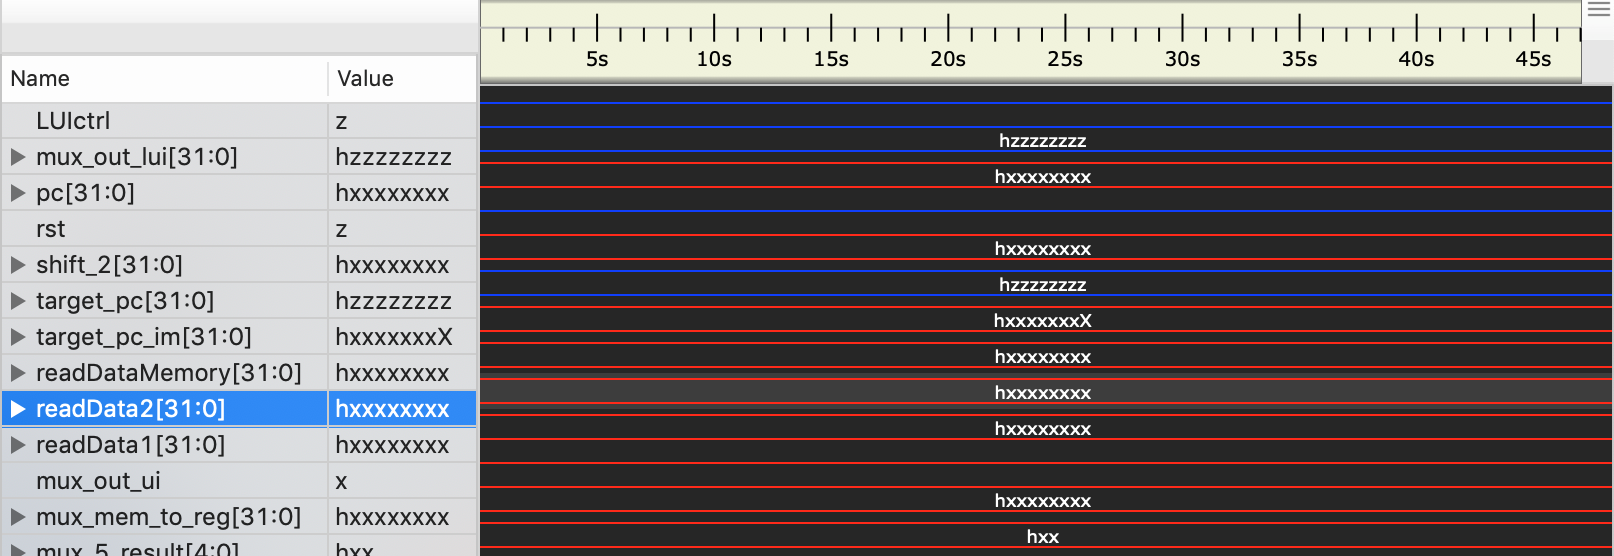
\includegraphics[scale=0.30]{images/jump_mux_error.png}
        \label{fig:jump-mux-error}
    \end{figure}
    
    To repair this crucial mistake we had to pass three auxiliary variables, again \textit{pc\_target} and the \textit{Jump} and \textit{Branch} signal form the Control editing the code like this
    
    \begin{lstlisting}
    module PC ( clk, pc, target_pc, 
                Jump, Branch);
    	input clk;
    	input [31:0] target_pc;
    	input Jump, Branch;
    	output reg [31:0] pc;
    
    	initial  begin
    		pc = 32'b0;
    	end
    
    	always @ (posedge clk) begin
    		pc = pc + 32'h4;
    		if (Jump || Branch)
    			pc = target_pc;
    	end
    endmodule
    \end{lstlisting}
    
    As this was mended everything worked just fine, we only needed to check if every instruction was working fine.
\section{Evaluation}
After creating each module we continued to the testing of every element individually, for this part we used ModelSim as the tester, this helped us to correct some syntax errors and other minor issues. The formulation of the test benches was after we had applied the necessary adjustments, simple values where logged in to the inputs to verify the veracity of the operation conducted by the component.Even with this tool some of the simple files couldn't be tested so along the \$display command we confirmed the results.

The next step was to pass the simulation, here everything got a lot harder, as the final phase of the evaluation things were suppose to work perfectly but the code was far from it; even if it did not have syntax errors and compiled fine, the processor did not carry out the task, initializing values to variables or losing data along the path.

In the \textit{Experimental Setup} there is a more detailed explanation of our principal mistakes in the process of creation.

\section{Conclusions}
Being students of Computer Science and adding to the equation that is our second year, we realize with this project the relevance of knowing what's really behind the compiler, how each instruction is executed and how much it cost to our computers to perform it by means of choosing instructions that now we know are the best for particular cases.  

For us the concept of programming wires was hard to grasp. However, once we understood it, we were able to cleanup our design and make it work. It was imperative to shift our usual thinking process for this new programming paradigm. In many instances we had to reuse wires and pass the same wires but with different values to modules which in regular programming would be nonsense.

The connection between the hardware and software was difficult to achieve, to the point where we needed to re-think simple processes and add new ones that we used to ignore, nevertheless, it's important to point out that this project was difficult to execute.

\section{Comments}
    We started to code the modules and compiling them separately without taking into consideration the other parts of the processor. Ergo, we underestimated the difficulty of the project.  
    
    We found it rewarding to learn new ways to approach at the hardware components using low level machine language. Also, we learned what was behind the system we were accustomed to use and why they worked the way they did.
    
    


\bibliographystyle{ieeetr}
\bibliography{bibliography}
\cite{1}
\cite{10.2307/29774812}
\cite{8326740}
\cite{unknown}


\end{document}
